\documentclass[12pt]{article}

\usepackage[a4paper]{geometry}
\geometry{left=2.5cm,right=2.5cm,top=2.5cm,bottom=2.5cm}

\usepackage{comment}
\usepackage{booktabs}
\usepackage{diagbox}
\usepackage{amsmath,amsfonts,graphicx,amssymb,bm,amsthm}
\usepackage{algorithm,algorithmicx}
\usepackage[noend]{algpseudocode}
\usepackage{fancyhdr}
\usepackage{subfigure} 
\usepackage{tikz}
\usepackage{graphicx}
\usetikzlibrary{arrows,automata}
\usepackage{hyperref}
\setlength{\headheight}{14pt}
\setlength{\parindent}{0 in}

\title{Proposal}
\usetikzlibrary{positioning}

\begin{document}
%\pagestyle{fancy}
%\lhead{Brown University}
%\chead{}
%\rhead{DATA 1030, 2021 Fall}

\begin{center}
	{\LARGE \bf DATA1030 Midterm Project Proposal}\\
	\vspace{0.3cm}{Nange Li, Oct. 11th 2021}
\end{center}

\section{Introduction}
% background
\subsection{Background}
Since the beginning of year 2020, the spreading coronavirus  disease 2019 (COVID-19) has aroused global concern on public health and people's lives. In order to closely monitor the nation-wise situation and reduce prevalence, many governments are trying to collect everyday data on new positive cases, death rate, and encouraging citizen to complete vaccinations. Under the travel-ban of several main countries and the fast increasing vaccination rate, the world actually witnessed an effect in combating the  spread. However, today our world is still under the threaten of COVID-19 pandemic. Predicting the future trend would be important as this is a base for short or long-term policies establishment.
\subsection{Dataset}
This project will employ the dataset maintained by {\em Our World in Data [1]} (OWID). While the data is fundamentally collected case-by-case, individual information regarding specific patients is not included in OWID's dataset. For each country or region, the daily-updated dataset has 65 columns, 122636 records (up to Oct 6th 2021) covering everyday updated COVID observations, demography statistics, as well as economical data of 233 countries.  Hence, this project will focus on the statistical information mined from the dataset, apply time series analysis and regression models to predict the future trend of total confirmed COVID-19 cases. \\

% previous works
Both mathematical models and machine learning models have been implemented by researchers on the OWID dataset. In 2020, Valvo et. al[2] developed a bimodal lognormal distribution model for the time distribution of deaths in a country. In the same year, Shreshth et. al[3] proposed a novel method using machine learning and cloud computing to improve the performance of pure mathematical models and predict the impact of the COVID-19 pandemic. They also applied the model on country-based data. 

\begin{figure}[htb]
	\setlength{\abovecaptionskip}{-1.cm}
	\centering
	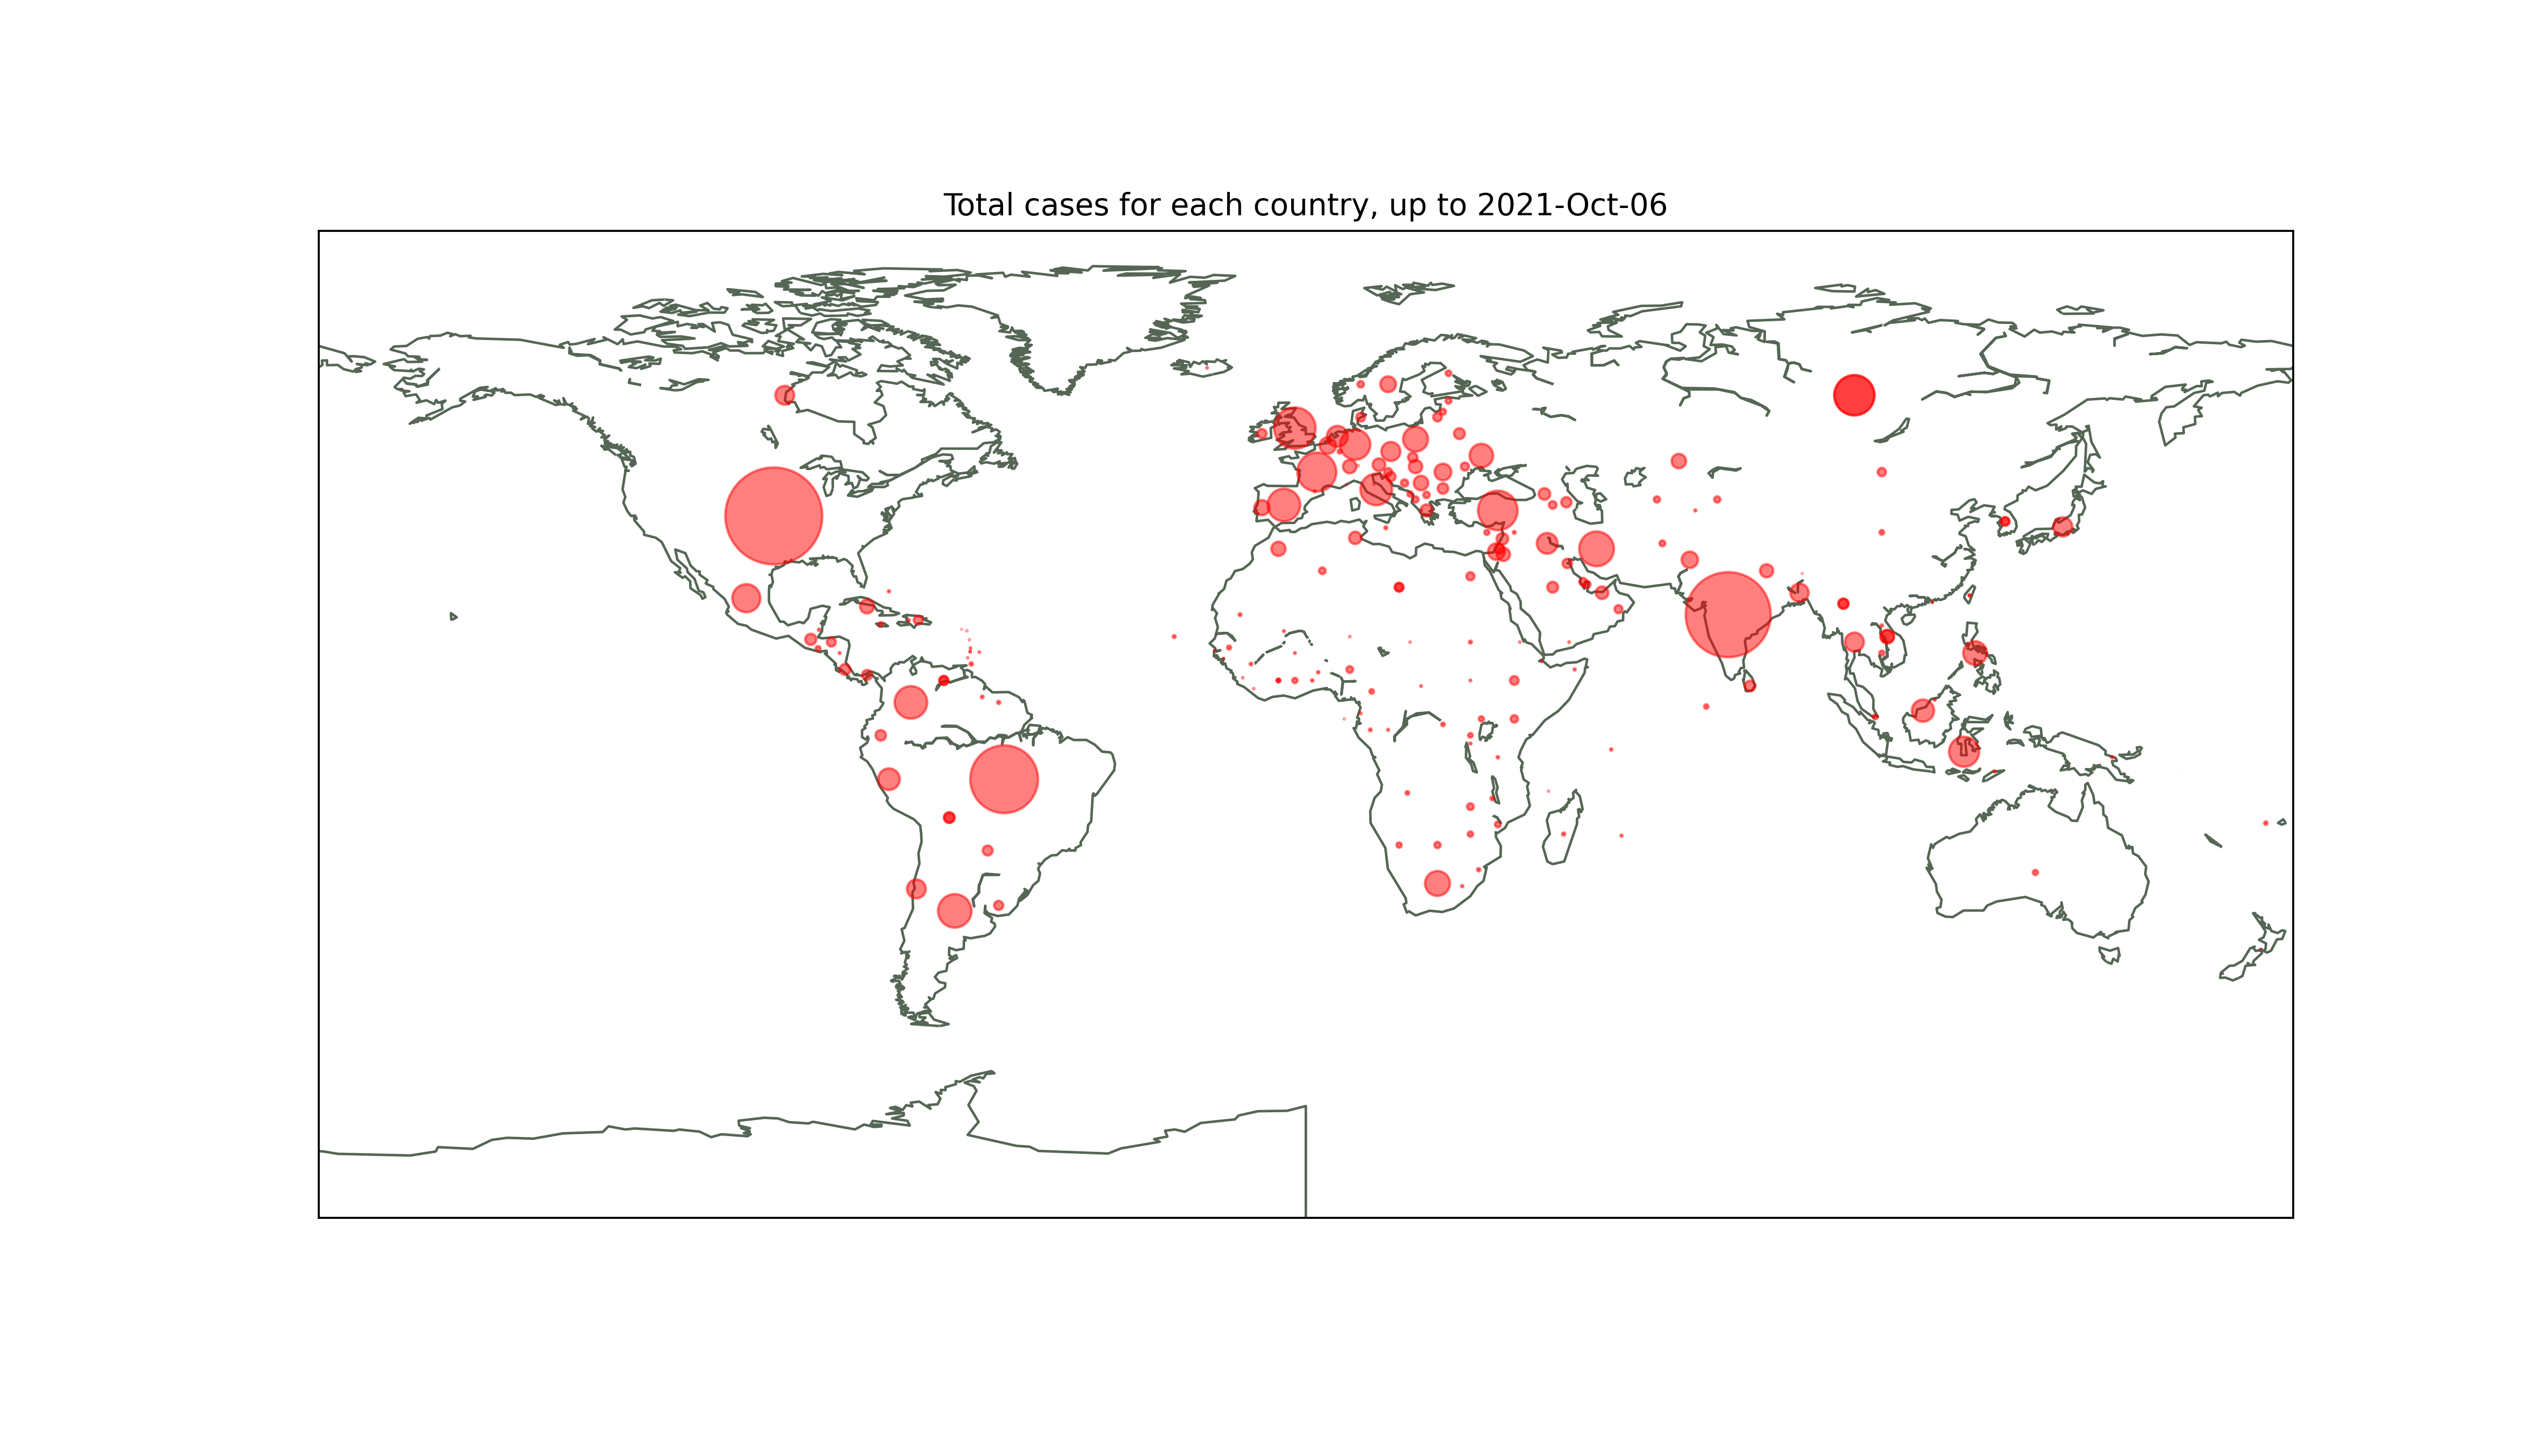
\includegraphics[width=0.7\linewidth]{../figures/total-cases-map.png} % Figure image
	\caption{This figure displays the total confirmed COVID-19 cases (up to Oct 6th 2021) of each country. Each red dot represents a country's total cases, placed at the averaged latitude and longitude. The size of the dot is the total cases number scaled by a factor of 30,000. From this figure, countries with the most total cases are the US, India and Brazil.} % Figure caption
\end{figure}

\section{Exploratory Data Analysis}
Figures 1-3 are included in this report visualizing the information extracted from a thorough 	EDA process. 

\begin{figure}[htb]
	\setlength{\abovecaptionskip}{-0.5cm}
	\centering
	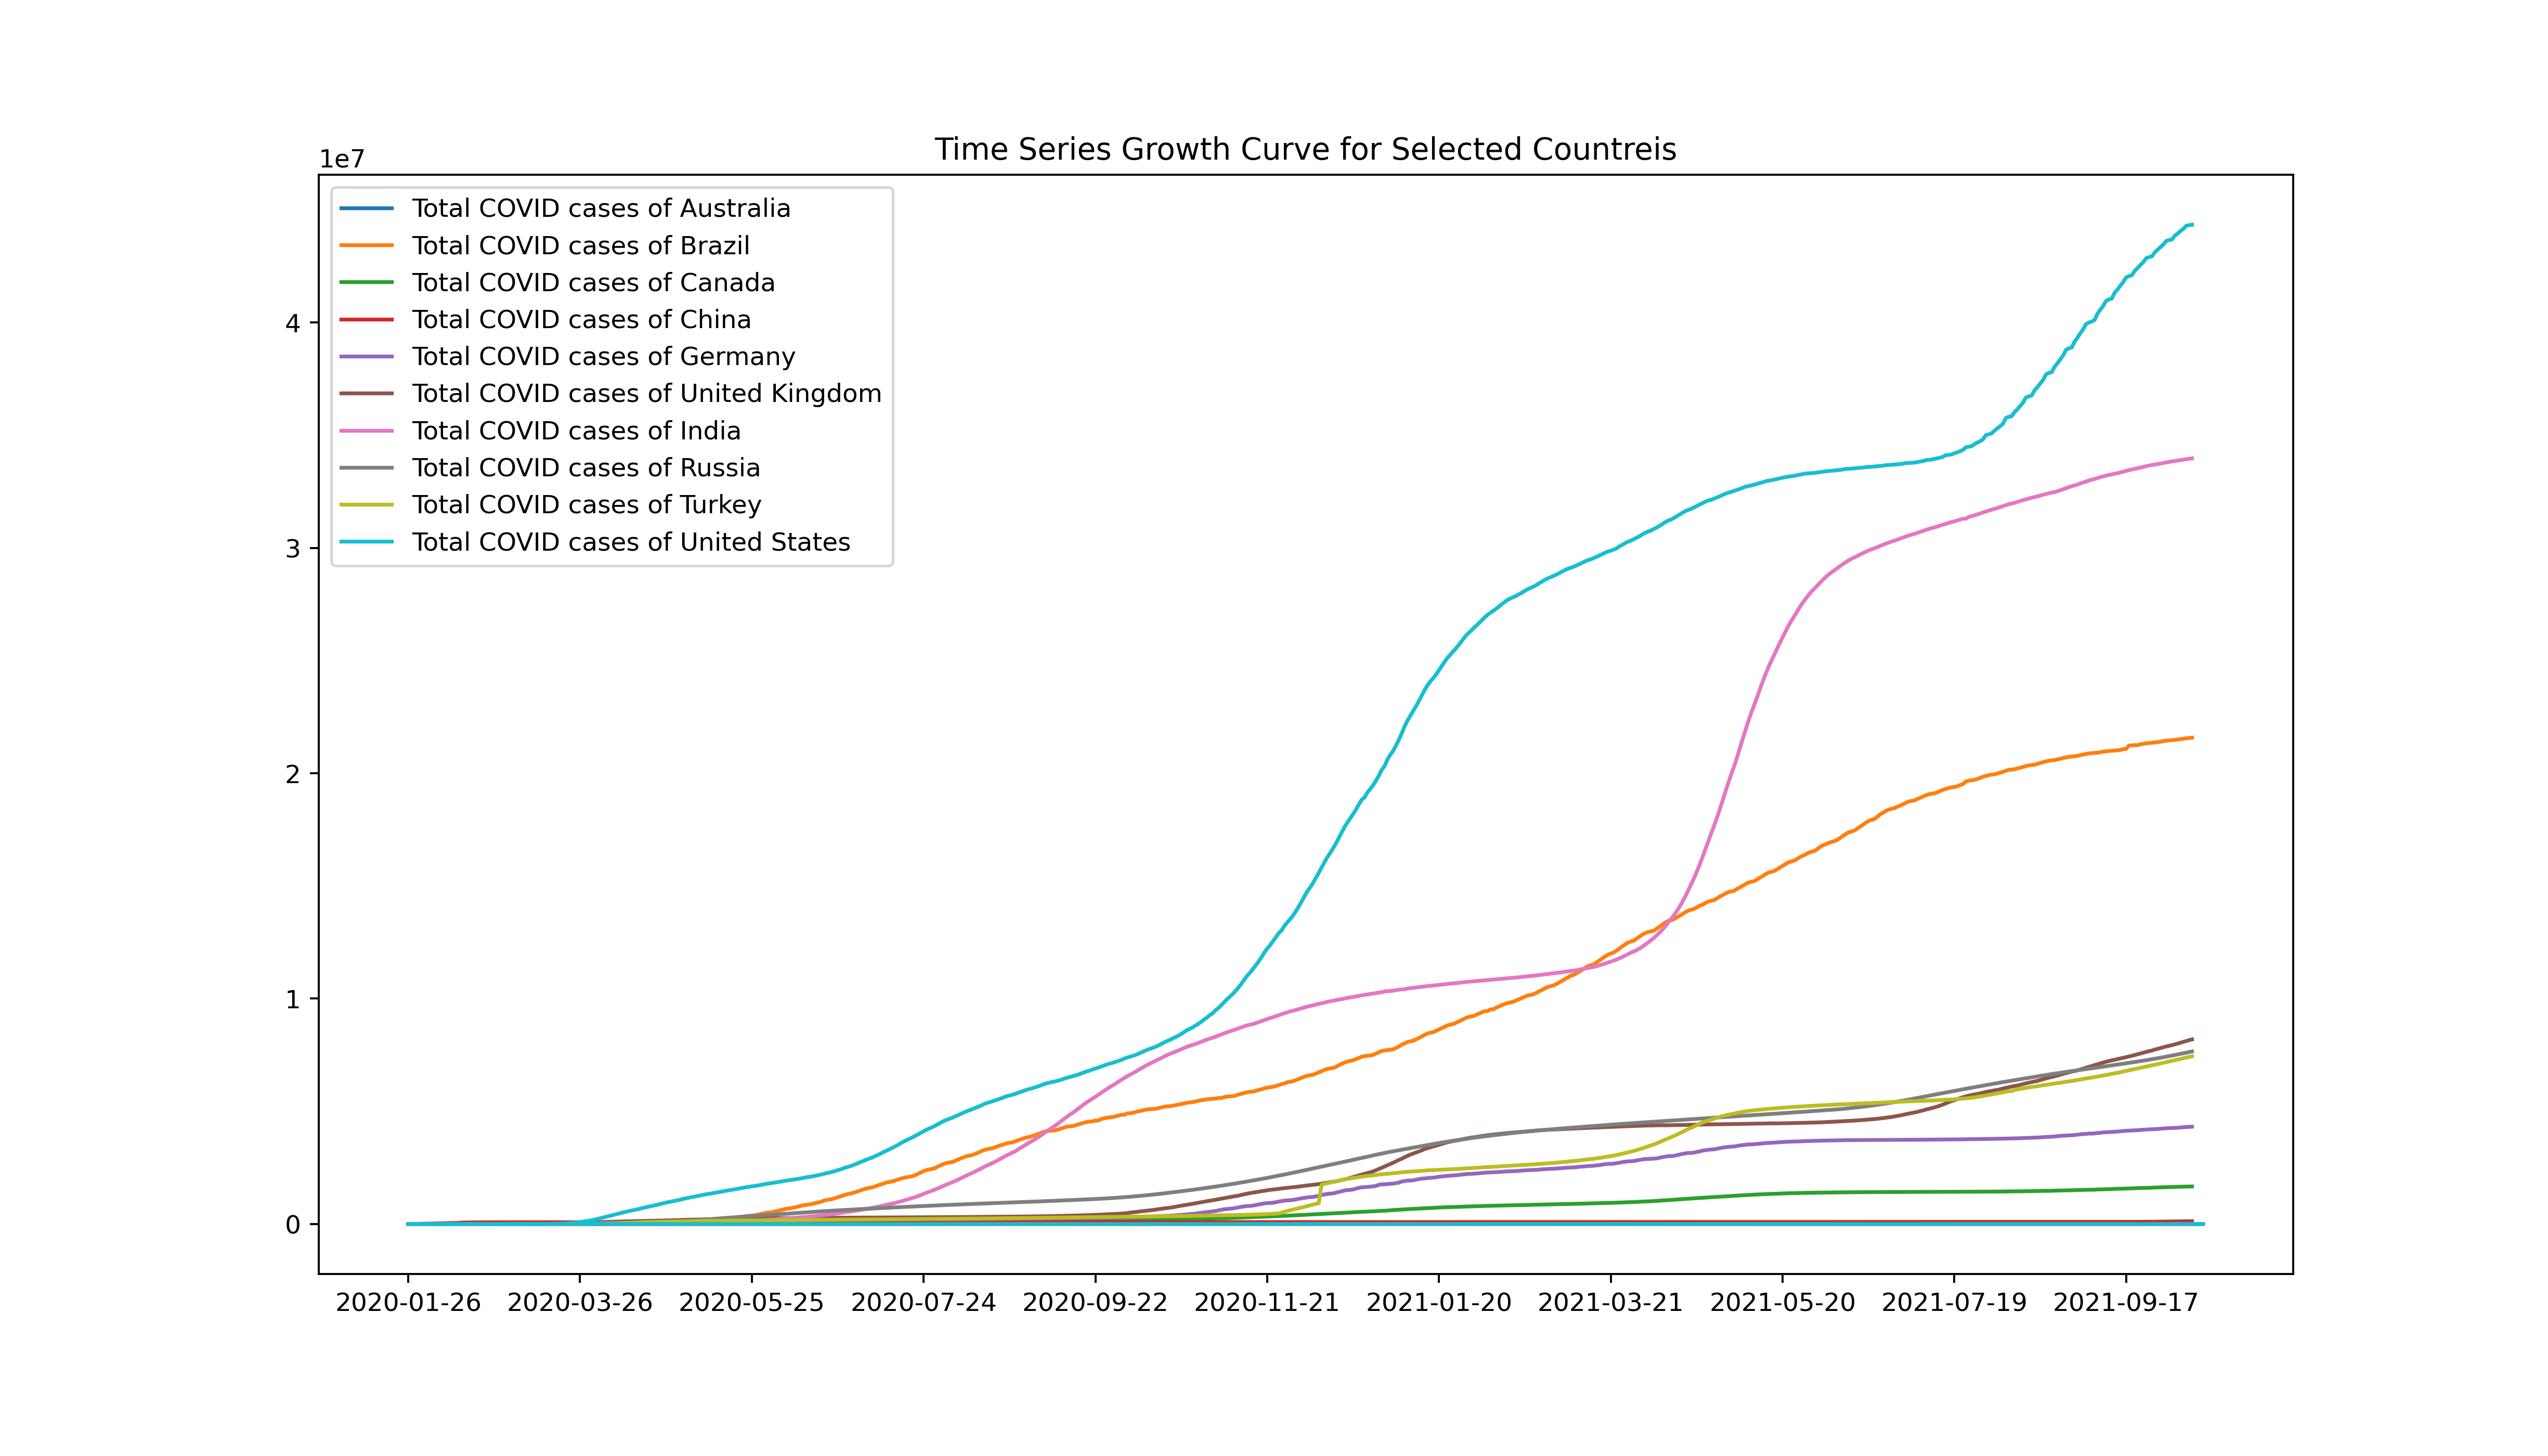
\includegraphics[width=0.7\linewidth]{../figures/total-cases-time-series.png} % Figure image
	\caption{Here ten countries are selected from 233, and this figure displays the growth curve of total cases from Jan 2020 to Oct 2021. While the curve of total cases of China, Australia, and even Canada, are kept relatively low and stable, the curve unfortunately goes up rapidly in the US, India and Brazil, which also accounts for their most cases in Figure 1.} % Figure caption
\end{figure}


\begin{figure}[htb]
	\centering
	\subfigure[total cases vs. new cases]{
		\label{total cases vs. new cases} 
		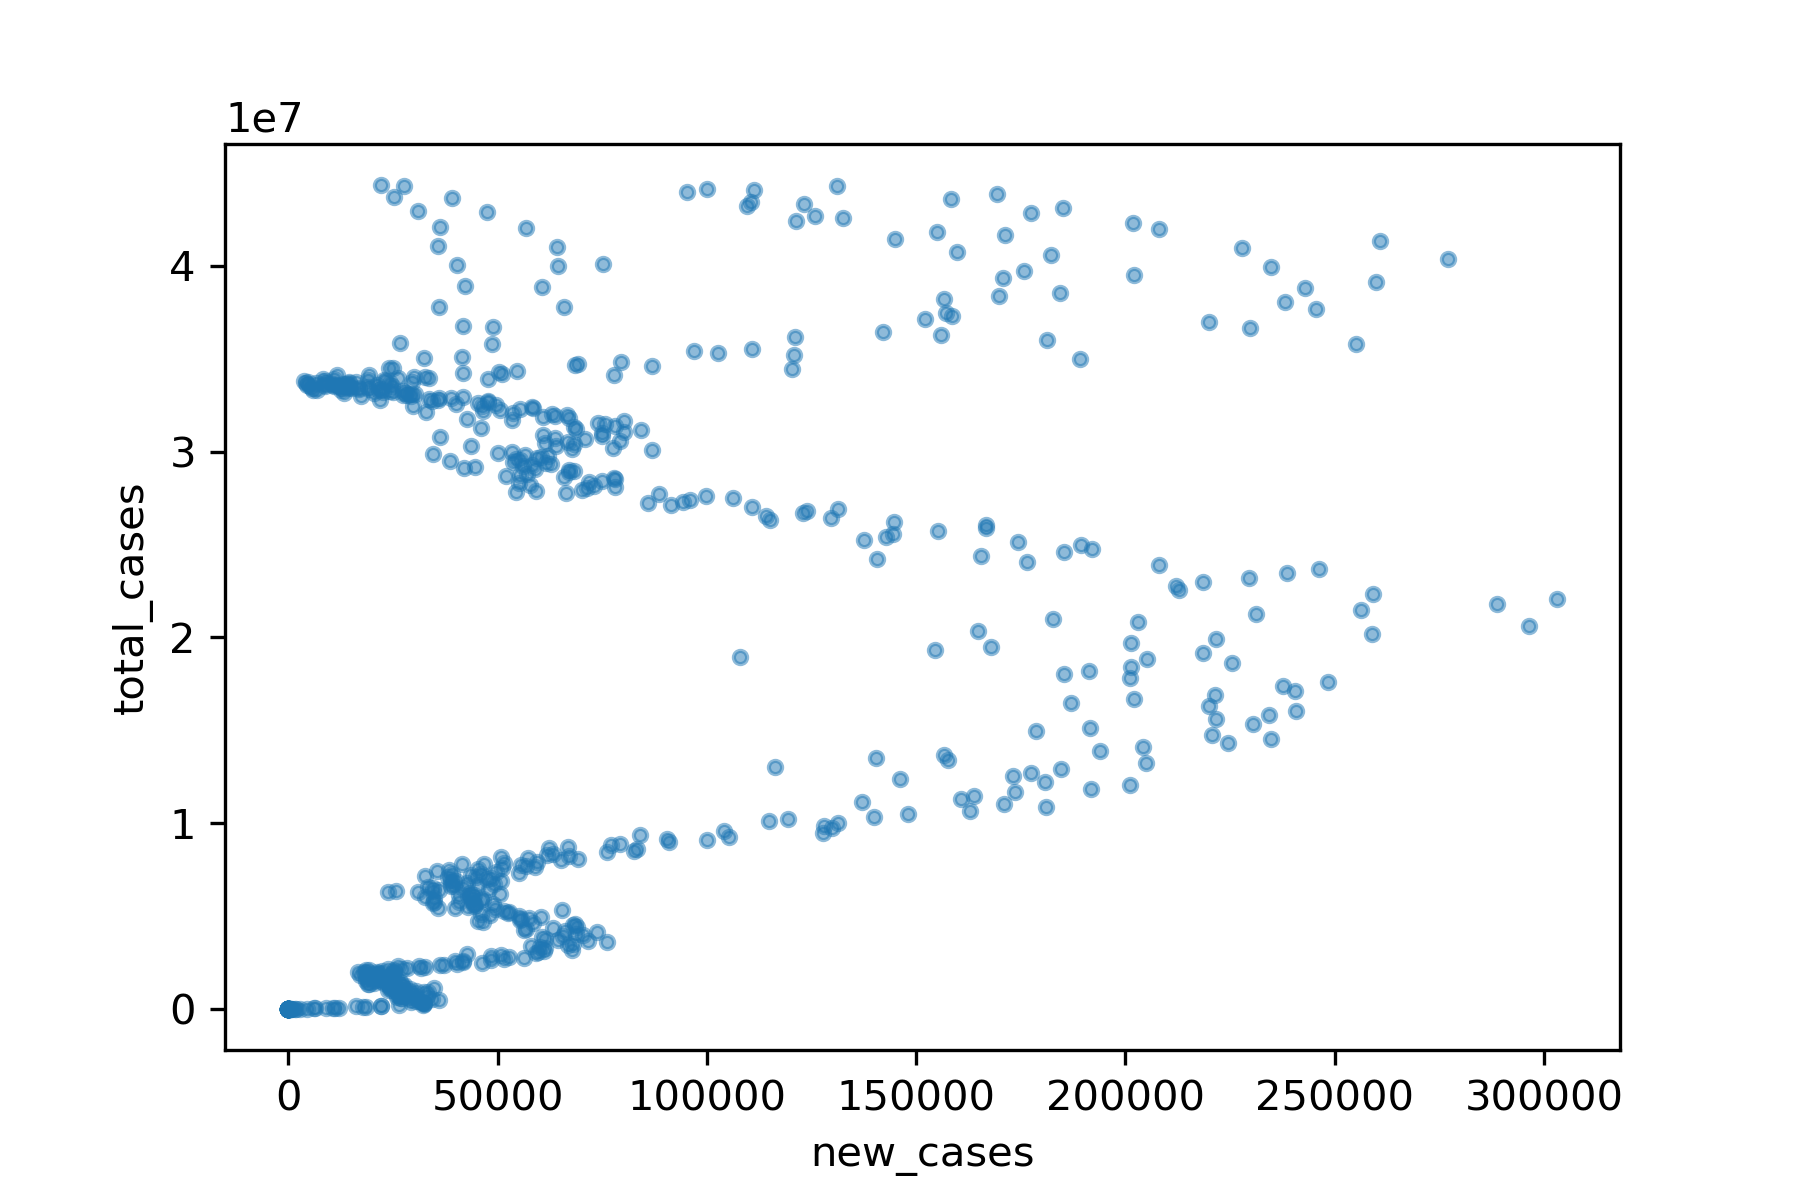
\includegraphics[width=0.45\textwidth]{../figures/total_cases-new_cases-scatter.png}}
	\subfigure[total cases vs. cumulated new cases]{	
		\label{total cases vs. cumulated new cases} %% label for secondsubfigure
		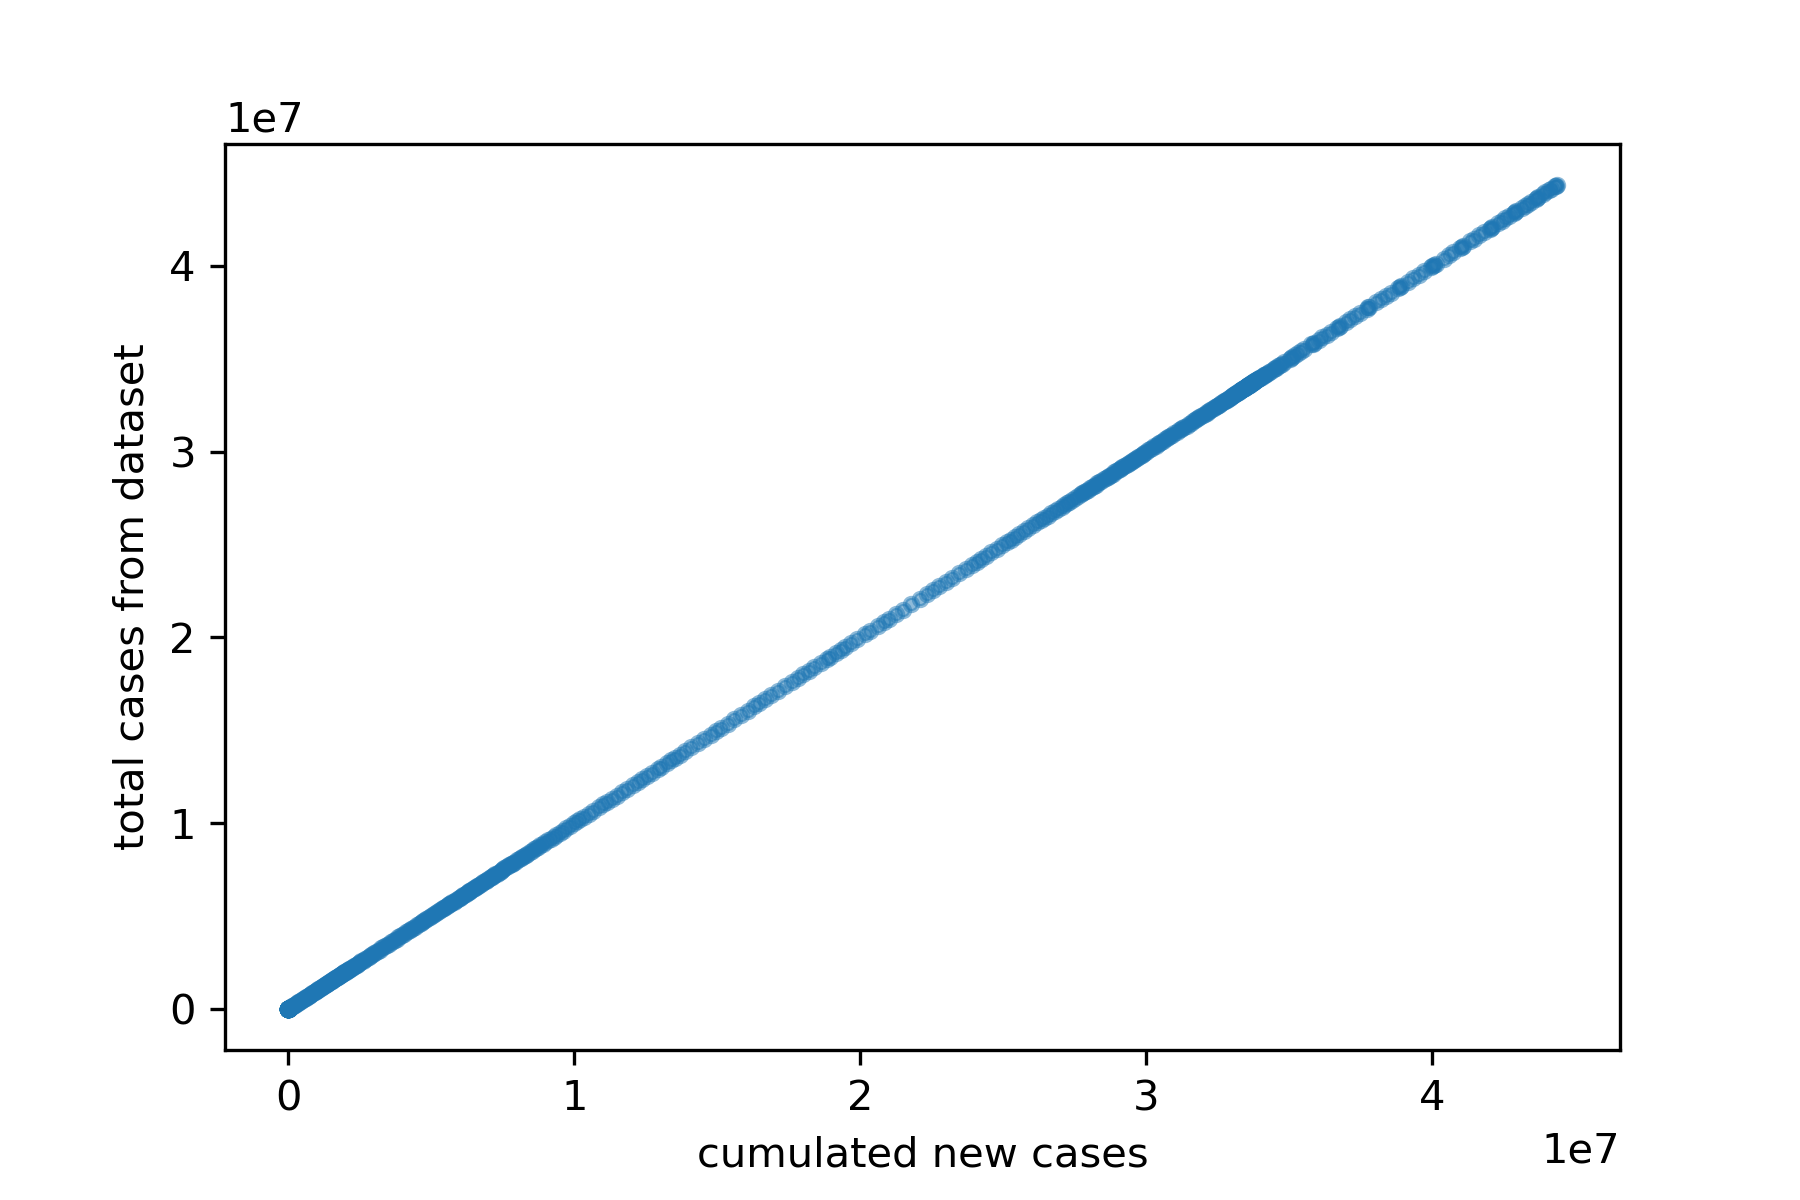
\includegraphics[width=0.45\textwidth]{../figures/total_cases-manual-scatter.png}}
	\caption{While there are 65 columns including our target variable of total cases and 64 feature variables, not all the features can be applied for future prediction. This figure shows a scatter between total cases and new cases data, with two variables convertible into each other - new cases series is the first-order difference of total cases series, and by cumulating the former one we can easily recover the latter series. Though from (a) it is not obvious to get this conclusion that the two series share the same information, after manually summing the new cases, (b) displays a straight line. (The Pearson correlation coefficient between manual cumulated new cases and total cases is exactly 1.0.)}
\end{figure}

\section{Modeling}
\subsection{Data Preprocessing}
For feature selection, the first three columns are indexing countries, so they are set as keys when grouping data. On the grouped set of one country, the date column is then set as index since the series has already been timely ordered. Also, columns directed connected to the target variable (those concerning new cases data) are eliminated from the selected features. After these steps, there are 54features elected for the following process.\\

As the dataset has a combination of group and time series structure, the splitting is performed on time series grouped by country names. For time series,  we should never use future information in validation or test, so the training set can only have records previous to records in the test set. 20\%  latest records are divided into test set, and in a loop for K-Fold, 80\% rest data in which one fraction consecutive to the training set is separated into validation set. StandardScaler is applied to the selected features when inside the loop of K-Fold. While there are features not strictly continuous, like the test cases and deaths only contain integers, it still makes sense to approximate those features with continuous variables instead of ordinal data, transferring the exact number to a kind of rate. 

\newpage
\begin{thebibliography}{99}
	\bibitem{1}Ritchie, H., Mathieu, E., et al. 2020. "Coronavirus Pandemic (COVID-19)". Published online at {\em OurWorldInData.org}. Retrieved from: \url{https://ourworldindata.org/coronavirus}
	\bibitem{2}Valvo, \& Paolo S. 2020. A Bimodal Lognormal Distribution Model for the Prediction of COVID-19 Deaths" {\em Applied Sciences }10, no. 23: 8500. \url{https://doi.org/10.3390/app10238500}
	\bibitem{3} Tuli, S., Tuli, R., Gil, S S., 2020. "Predicting the growth and trend of COVID-19 pandemic using machine learning and cloud computing". {\em Internet of Things},
	Volume 11,
	2020,
	100222,
	ISSN 2542-6605,
	\url{https://doi.org/10.1016/j.iot.2020.100222}.
\end{thebibliography}
	
\end{document}

